%!TEX program = xelatex
\documentclass[12pt,a4paper,utf8]{ctexart}
\usepackage{graphicx}
\usepackage{amsmath}
\usepackage{amssymb}
\usepackage{subfig}
\usepackage{cite}
\usepackage[ntheorem]{empheq}
\usepackage{enumitem}
\usepackage{fullpage}
\usepackage{cleveref}
\usepackage{cellspace}
\usepackage{listings}
\usepackage{color}
\definecolor{gray}{rgb}{0.5,0.5,0.5}
\definecolor{dkgreen}{rgb}{.068,.578,.068}
\definecolor{dkpurple}{rgb}{.320,.064,.680}

% set Matlab styles
\lstset{
   language=Matlab,
   keywords={break,case,catch,continue,else,elseif,end,for,function,
      global,if,otherwise,persistent,return,switch,try,while},
   basicstyle=\ttfamily,
   keywordstyle=\color{blue}\bfseries,
   commentstyle=\color{dkgreen},
   stringstyle=\color{dkpurple},
   backgroundcolor=\color{white},
   tabsize=4,
   showspaces=false,
   showstringspaces=false
}

\begin{document}

\CJKfamily{zhkai}       


\begin{center}
\textbf{作业一}\\
\textbf{林成渊 ~~~~~ PB18051113 ~~~~~ \zhtoday}\\
\end{center}
\textit{}
\vspace{\baselineskip}

\begin{enumerate}
\item[第一题] \textbf{重心插值公式(barycentric interpolation formula)}  

课堂上我们已经讨论过了基于$n+1$个插值点$\{x_j\}_{j=0}^n$的Lagrange插值多项式:
\begin{equation}
p(x) = \sum_{j=0}^{n} f_j \ell_j(x) \label{lagrange}
\end{equation}
此处,$f_j = f(x_j)$。Lagrange插值基函数(Lagrange polynomial)
\begin{equation}
\ell_{j}(x)=\frac{\prod_{k \neq j}\left(x-x_{k}\right)}{\prod_{k \neq j}\left(x_{j}-x_{k}\right)} \label{cardinal}
\end{equation}
满足
\begin{equation}
\ell_{j}\left(x_{k}\right)=\left\{\begin{array}{ll}
1 & k=j \\
0 & k \neq j
\end{array}\right. \nonumber
\end{equation}

(a)首先证明Lagrange基函数可以用节点多项式简洁地表示出来,根据节点多项式的表达式:
\begin{equation}
\ell_(x) = \prod_{k=0}^{n} (x-x_{k}) \nonumber
\end{equation}
求导得:
\begin{equation}
\ell_j'(x) = \sum_{i=0}^n \frac{\prod_{k=0}^n (x-x_k)}{(x-x_i)} \nonumber
\end{equation}
代入$x=x_{j}$得到:
\begin{equation}
\ell_j'(x_j) =  \prod_{k \neq j}\left(x_j-x_k\right) \nonumber
\end{equation}
所以有
\begin{equation}
   \begin{aligned}
   \ell_j(x) &= \frac{\prod_{k \neq j}\left(x-x_k\right)}{\prod_{k \neq j}\left(x_j-x_k\right)} \\
   &= \frac{\prod_{k=0}^n (x-x_k)}{\ell'(x_j) (x-x_j)} \\
   &= \frac{\ell (x)}{\ell'(x_j) (x-x_j)} \nonumber
   \end{aligned}
\end{equation}
证毕。接下来推导重心插值公式的第一形式:
\begin{equation}
   \begin{aligned}
   p(x) &= \sum_{j=0}^n f_j \ell_j(x) \\ \nonumber
   &= \sum_{j=0}^n f_j \frac{\ell (x)}{\ell'(x_j) (x-x_j)} \\ \nonumber
   &= \ell (x) \sum_{j=0}^n \frac{f_j}{(x-x_j)\ell '(x_j)} \\ \nonumber
   &= \ell (x) \sum_{j=0}^n \frac{\lambda_j}{x-x_j} f_j,\qquad \lambda_j = \frac{1}{\ell '(x_j)} \nonumber
   \end{aligned}
\end{equation}
(b)观察(1),接下来证明所有Lagrange基函数的和恰好为1。
首先能看到Lagrange插值基函数只与插值点的选取有关,而与具体的函数无关。
那么,式子(1)的成立应当与具体函数$f$的选取无关,于是选取$f\equiv 1$,有:
\begin{equation}
f(x)\equiv 1,\qquad p(x) = \sum_{j=0}^n\ell_j(x) \nonumber
\end{equation}
由余项定理可知,$p(x) = 1$
\begin{equation}
p(x) = \sum_{j=0}^n\ell_j(x)  = 1 \nonumber
\end{equation}
证毕。接下来推导重心插值公式的第二形式,首先有
\begin{equation}
   \begin{aligned}
      \ell_j(x)&= \frac{\ell (x)}{\ell'(x_j) (x-x_j)} \\ \nonumber
      &= \frac{\ell (x) \lambda _j}{x-x_j} \nonumber
   \end{aligned}
\end{equation}
对等式两边求和,由所有Lagrange基函数的和为1,有
\begin{equation}
   \begin{aligned}
      1 &= \sum_{j=0}^n \ell_j(x) \\ \nonumber
      &= \sum_{j=0}^n \frac{\ell (x) \lambda _j}{x-x_j} \\ \nonumber
      &= \ell (x) \sum_{j=0}^n \frac{\lambda _j}{x-x_j} \nonumber
   \end{aligned}
\end{equation}
得到等式
\begin{equation}
   \ell (x) = 1 \bigg/ \sum_{j=0}^n \frac{\lambda _j}{x-x_j} \nonumber
\end{equation}
将其代入重心插值公式的第一形式即得
\begin{equation}
   \begin{aligned}
   p(x) &= \ell (x) \sum_{j=0}^n \frac{\lambda_j}{x-x_j} f_j \\ \nonumber
   &= \sum_{j=0}^n \frac{\lambda_j f_j}{x-x_j} \bigg/ \sum_{j=0}^n \frac{\lambda _j}{x-x_j} \nonumber
   \end{aligned}
\end{equation}

(c)推导取Chebyshew点作为插值点时插值权重$\lambda _j$的化简,首先讨论$1\le j \le n-1$的情形,有
\begin{equation}
   \begin{aligned}
      \lambda_j &= 1 \bigg/ \ell '(x_j) \\ \nonumber
      &= 1 \bigg/ \prod_{k \neq j} (x_j - x_k) \\ \nonumber
      &= 1 \bigg/ \prod_{k \neq j} [cos(j\pi /n)-cos(k\pi /n)] \\ \nonumber
      &= 1 \bigg/ \prod_{k \neq j} [-2sin(\frac{j+k}{2n} \pi)sin(\frac{j-k}{2n} \pi)] \\ \nonumber
      &= (-1)^{j-1} sin(\frac{j}{n} \pi )\bigg/ -2sin(\frac{j}{2n} \pi )cos(\frac{j}{2n} \pi )\prod_{k=1}^{2n-1} sin(\frac{k}{2n} \pi ) \\ \nonumber  
      &= (-1)^j \bigg/ \prod_{k=1}^{2n-1} sin(\frac{k}{2n} \pi ) \\ \nonumber
      &= \frac{2^{n-1}}{n} (-1)^j \nonumber
   \end{aligned}
\end{equation}
$j=0$或$j=n$情况下无需考虑j的正负情况,同理可得
\begin{equation}
   \lambda_0 = \frac{2^{n-2}}{n} ,\qquad \lambda_n = \frac{2^{n-2}}{n}(-1)^n \nonumber
\end{equation}

(d)基于Chebyshev点进行插值,\textsc{Matlab}程序显示如下:
\begin{lstlisting}[frame=single]
clear, clc, clf
LW = 'linewidth'; lw = 2;
%%
n = 5000;
nset = linspace(0,n,n+1)';
x = cos(nset * pi /n);
m = 10000;
xx = linspace(-1, 1, m+1)';
F = @(x) tanh(20 * sin(12 * x)) 
         + 0.02 * exp(3 * x) .* sin(300 * x);
f = F(x);
%%
p = zeros(m+1, 1);
R = ones(m, 1);
for k = 1:m+1
    S_deno = zeros(n+1,1);
    S_nume = zeros(n+1,1);
    for t = 1:n+1
        if (xx(k) == x(t))
            S_deno(t) = 0;
        else
            S_deno(t)= (-1)^t / (xx(k)-x(t));
        end
    end
    S_deno(1) = S_deno(1) / 2;
    S_deno(n+1) = S_deno(n+1) / 2;
    S_nume = S_deno .* f;
    p(k) = sum(S_nume) / sum(S_deno);
end
%%
figure(1)
subplot(2,1,1);
plot(xx, F(xx), 'k', LW, lw), hold on
plot(xx, p,'--', LW, lw)
legend('exact', 'interpolant', 'location', 'nw')
subplot(2,1,2)
semilogy(xx, abs(F(xx) - p), 'k', LW, lw), hold on
legend('error',  'location', 'se')
\end{lstlisting}
使用该程序进行插值作图得到图1
\begin{figure}[htbp]
        \centering
        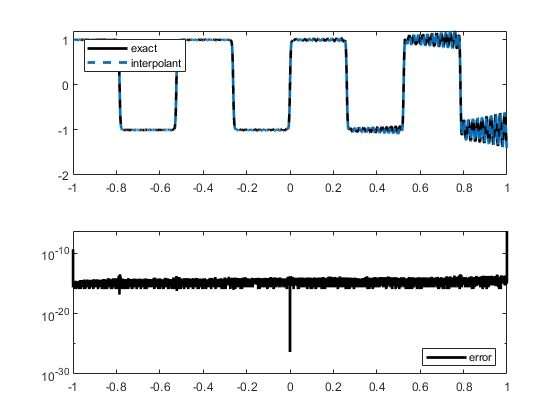
\includegraphics[width=0.7\textwidth]{image/T1.png}
        \caption{第一题(d)小题作图结果}
\end{figure}

\item[第二题]
考虑到(c)图和程序是(a)的扩展版本,为了方便起见,合并(a)(c),直接给出最终实现的程序和图像 此处先给出对(b)的解释

(b)log表征的是其值的数量级变化,
在基于多项式的数据拟合中,最大误差的数量级近似地等同于误差级数的主要项的指数,
而图中所反映的,误差最大值随着n的取值不同的趋向在loglog图上近似于线性,
由于n是由2的k次方生成的,
也就是说,增加采样点的数量级,误差的数量级也会近似同比率地变化,
而这里的斜率反应的就是变化的比率。这与先前所述多项式拟合的数据误差是一致的,
它正比于误差级数中的最大项的系数


(a/c)\textsc{Matlab}程序显示如下:
\begin{lstlisting}[frame=single]
clear, clc, clf
LW = 'linewidth'; lw = 2;
inf_k = 6; sup_k = 12;
F = @(x) exp(3.*cos(pi.*x));
%%
kgroup = (inf_k:sup_k);
ngroup = 2.^kgroup;
for i = 1:(sup_k-inf_k+1)
    k = kgroup(i);
    n = ngroup(i);
    x = linspace(-1, 1, n+1)';    
    f = F(x);
%%
    h = diff(x);
    df = diff(f);
    lambda = h(2:n) ./ (h(2:n) + h(1:n-1));
    d = 6 * ( df(2:n) ./ h(2:n) 
        - df(1:n-1) ./ h(1:n-1) ) ./ (h(2:n) 
        + h(1:n-1));
    mu = 1-lambda;
%%
    %第一类边界条件
    M0 = 0;
    Mn = 0;
    A1 = diag(2*ones(n-1,1)) + diag(lambda(1:n-2), 1) 
         + diag(mu(2:n-1), -1);
    D1 = [d(1) - mu(1)*M0; d(2:n-2); 
           d(n-1) - lambda(n-1)*Mn];
    M1 = A1\D1;
    M1 = [M0; M1; Mn];
%%
    %第二类边界条件
    m0 = 0;
    mn = 0;
    lambda2 = [1; lambda];
    mu2 = [mu; 1];
    d0 = 6 * ( df(1) / h(1) - m0 ) / h(1);
    dn = 6 * ( mn - df(n) / h(n) ) / h(n);
    D2 = [d0; d; dn];
    A2 = diag(2*ones(n+1,1)) + diag(lambda2, 1) 
         + diag(mu2, -1);
    M2 = A2\D2;
%%
    %第三类边界条件
    lambda0 = h(1) / (h(1) + h(n));
    lambda3 = [lambda0; lambda(1:n-2)];
    mu0 = 1 - lambda0;
    d0 = 6 * (df(1) ./ h(1) - df(n) ./ h(n)) 
         / (h(1) + h(n));
    D3 = [d0; d];
    A3 = diag(2*ones(n,1)) + diag(lambda3, 1) 
         + diag(mu, -1);
    A3(1, n) = mu0;
    A3(n, 1) = lambda(n-1);
    M3 = A3\D3;
    M3 = [M3; M3(1)];
%%
    S1(i) = CubicSpline(x, F, h, M1);
    S2(i) = CubicSpline(x, F, h, M2);
    S3(i) = CubicSpline(x, F, h, M3);
    
end
figure(1)
p1 = loglog(ngroup, S1, 'r'); hold on
p2 = loglog(ngroup, S2, '--k'); hold on
p3 = loglog(ngroup, S3, '-.b'); hold on
legend('situation 1', 'situation 2', 'situation 3', 
       'location','best')
%%
function S = CubicSpline(x, F, h, M)
LW = 'linewidth'; lw = 2;
n = size(x) - 1;
f = F(x);
for k = 1:n
    m = 4;
    xx = linspace(x(k), x(k+1), m+2)';
    S = ( (x(k+1)-xx).^3*M(k) + (xx-x(k)).^3*M(k+1) ) 
        / (6*h(k)) +...
        ( (x(k+1)-xx)*f(k) + (xx-x(k))*f(k+1) ) 
        / h(k) -...
        h(k) * ( (x(k+1)-xx)*M(k) + (xx-x(k))*M(k+1) ) / 6;
    error = abs(F(xx) - S);
    errorp(m*k-m+1:m*k) = error(2:end-1);
end
S = max(errorp);
end
\end{lstlisting}

使用该程序进行插值作图得到图2
\begin{figure}[htbp]
        \centering
        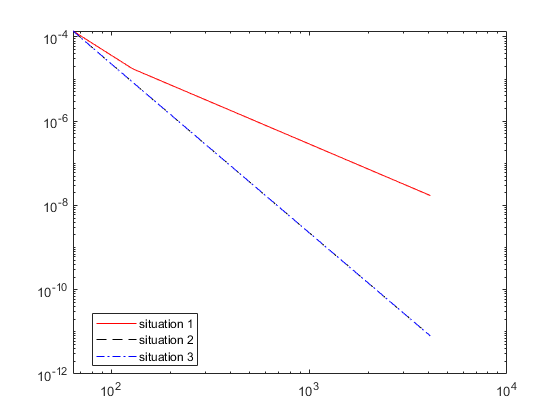
\includegraphics[width=0.7\textwidth]{image/T2.png}
        \caption{第二题(a/c)小题作图结果}
\end{figure}

\item[第三题]
对下列数据用最小二乘法求形如$y=ae^{bx}$的经验公式

\begin{tabular}{ccccc}
\hline
$x_i$& -0.70& -0.50& 0.25& 0.75\\
\hline
$y_i$& 0.99& 1.21& 2.57& 4.23\\
\hline
\end{tabular}

首先计算$z_i = lny_i$,令$a'=lna$,再对数据$(x_i,z_i)$作线性拟合$z=a'+bx$,详细过程由程序自动推演

\textsc{Matlab}程序显示如下:
\begin{lstlisting}[frame=single]
clear, clc, clf

x = [-0.70,-0.50,0.25,0.75];
y = [0.99,1.21,2.57,4.23]';
z = log(y);
sizem = length(x); 
%%
%定义矩阵A
A = [ones(sizem,1), x'];
%计算矩阵A'A和A'Y
M = A'*A;
Z = A'*z;
%解方程A'Aa=A'Y
result = M\Z;
a=exp(result(1));
b=result(2);
%%
%分析误差
F = @(x) a * exp(b*x);
f = F(x);
AbsPoor = abs(f' - y);
error = sqrt(sum(AbsPoor.^2));
%输出
figure(1);
plot(x,y,'o'); hold on
fplot(F,'k',[-2,2]);
legend('sampling point', 'fitted curve', 
       'location', 'best')
disp(a);
disp(b);
disp(error);
\end{lstlisting}
运行程序得到输出结果$a=1.9972,b=1.0020$,2-范数为$0.0062$,绘制图像如图3
\begin{figure}[htbp]
        \centering
        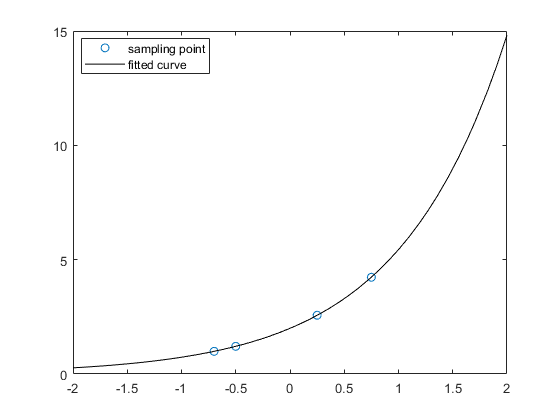
\includegraphics[width=0.5\textwidth]{image/T3.png}
        \caption{第三题作图结果}
\end{figure}
\end{enumerate}




\end{document}
